\documentclass[12pt,a4paper]{article}
\usepackage[utf8]{inputenc}
\usepackage{amsmath}
\usepackage{amsfonts}
\usepackage{amssymb}
\usepackage{hyperref}
\usepackage{graphicx}
\usepackage[a4paper]{geometry}
\usepackage{fullpage}
\author{Gergely Imreh}
\title{Zeeman slower summary}
\date{\today, v1}
\begin{document}

\maketitle

\section{Introduction}

The purpose of this document to summarize our simulation and construction results of the Zeeman slower in our lab.

\section{Theory}

\subsection{Field shape}

\begin{equation}
a(z) = -\frac{\hbar k \Gamma}{2 m} \frac{s}{1 + s + 4 \delta(z)^2 / \Gamma^2}
\label{eq:accel}
\end{equation}
where $s$ is $I/I_{\rm sat}$ saturation parameter. The assumed maximum deceleration is at $s \rightarrow \infty$, and at $\delta = 0$ we have $\eta = \frac{s}{1 + s}$.

The detuning is 
\begin{equation}
\delta(z) = k v(z) + \Delta - \frac{\mu'}{\hbar} B(z)
\end{equation}
where 
\begin{equation}
\mu' = \mu_{B}(g_e m_e - g_g m_g)
\end{equation}
and in our case $\mu' = \mu_{B}$.

Most people use the ``ideal'' field profile, assuming constant deceleration (e.g adapted from \cite{Bell2010}):
\begin{equation}
B_{\rm ideal}(z) = \frac{\hbar k}{\mu'}\sqrt{v_0^2 + 2 \eta a_m z} + B_a
\label{eq:bideal}
\end{equation}
where $\eta$ is the cooling efficiency, $v_0$ is the maximum capture velocity chosen (or fixed by a given slower length and $\eta$), $a_m = -\frac{\hbar k \Gamma}{2 m}$ is the maximum deceleration, from Eq. \ref{eq:accel} setting $s = \infty$, and $B_a$ is a bias field, or an equivalent laser detuning from the resonance as $B_a = \frac{\hbar}{\mu'} \Delta$.

In this case the magnetic field gradient is
\begin{equation}
\frac{\partial B_{\rm ideal}}{\partial z} = \frac{\hbar k}{\mu'} \frac{\eta a_m}{\sqrt{v_0^2 + 2 \eta a z}}
\end{equation}
which is a negative number because $a_m < 0$.

From Eq. \ref{eq:accel} and \ref{eq:bideal} one can deduce that the efficiency is
\begin{equation}
\eta = \frac{s}{1 + s}
\end{equation}

\subsection{Detuning}

The detuning at a given position is given by three contribution as
\begin{equation}
\delta = k v + \Delta - \frac{\mu'}{\hbar} B
\end{equation}
where v is the atomic velocity.

\begin{equation}
\frac{\partial \delta}{\partial z} = k \frac{\partial v}{\partial z} - \frac{\mu'}{\hbar}\frac{\partial B}{\partial z} = k \frac{\partial v}{\partial t} \frac{1} {\frac{\partial z}{\partial t}} - \frac{\mu'}{\hbar}\frac{\partial B}{\partial z}
= k \frac {a}{v} - \frac{\mu'}{\hbar}\frac{\partial B}{\partial z}
\label{eq:dddz}
\end{equation}

Without change in the magnetic field (that is zero gradient), there's always just going to lower detuning. On the other hand, when there's $\partial B/\partial z < 0$: the can be stable and unstable points: either 1 stable and 2 unstable, or 1 unstable if $|\partial B / \partial z| >> 0$ (set a more correct level for this).


Figure \ref{fig:dddz1} shows the spatial gradient of the detuning $\partial \delta / \partial z$ for a set of commonly used parameters and assuming a constant magnetic field. The gradient is negative in the entire region, meaning that the detuning is moving to the red. Given the parameters, that means $\partial v / \partial z < 0$, which is deceleration. Given the profile, the deceleration is the largest near the resonance, and away from it is decreasing rapidly.

\begin{figure}[htb]
\centering
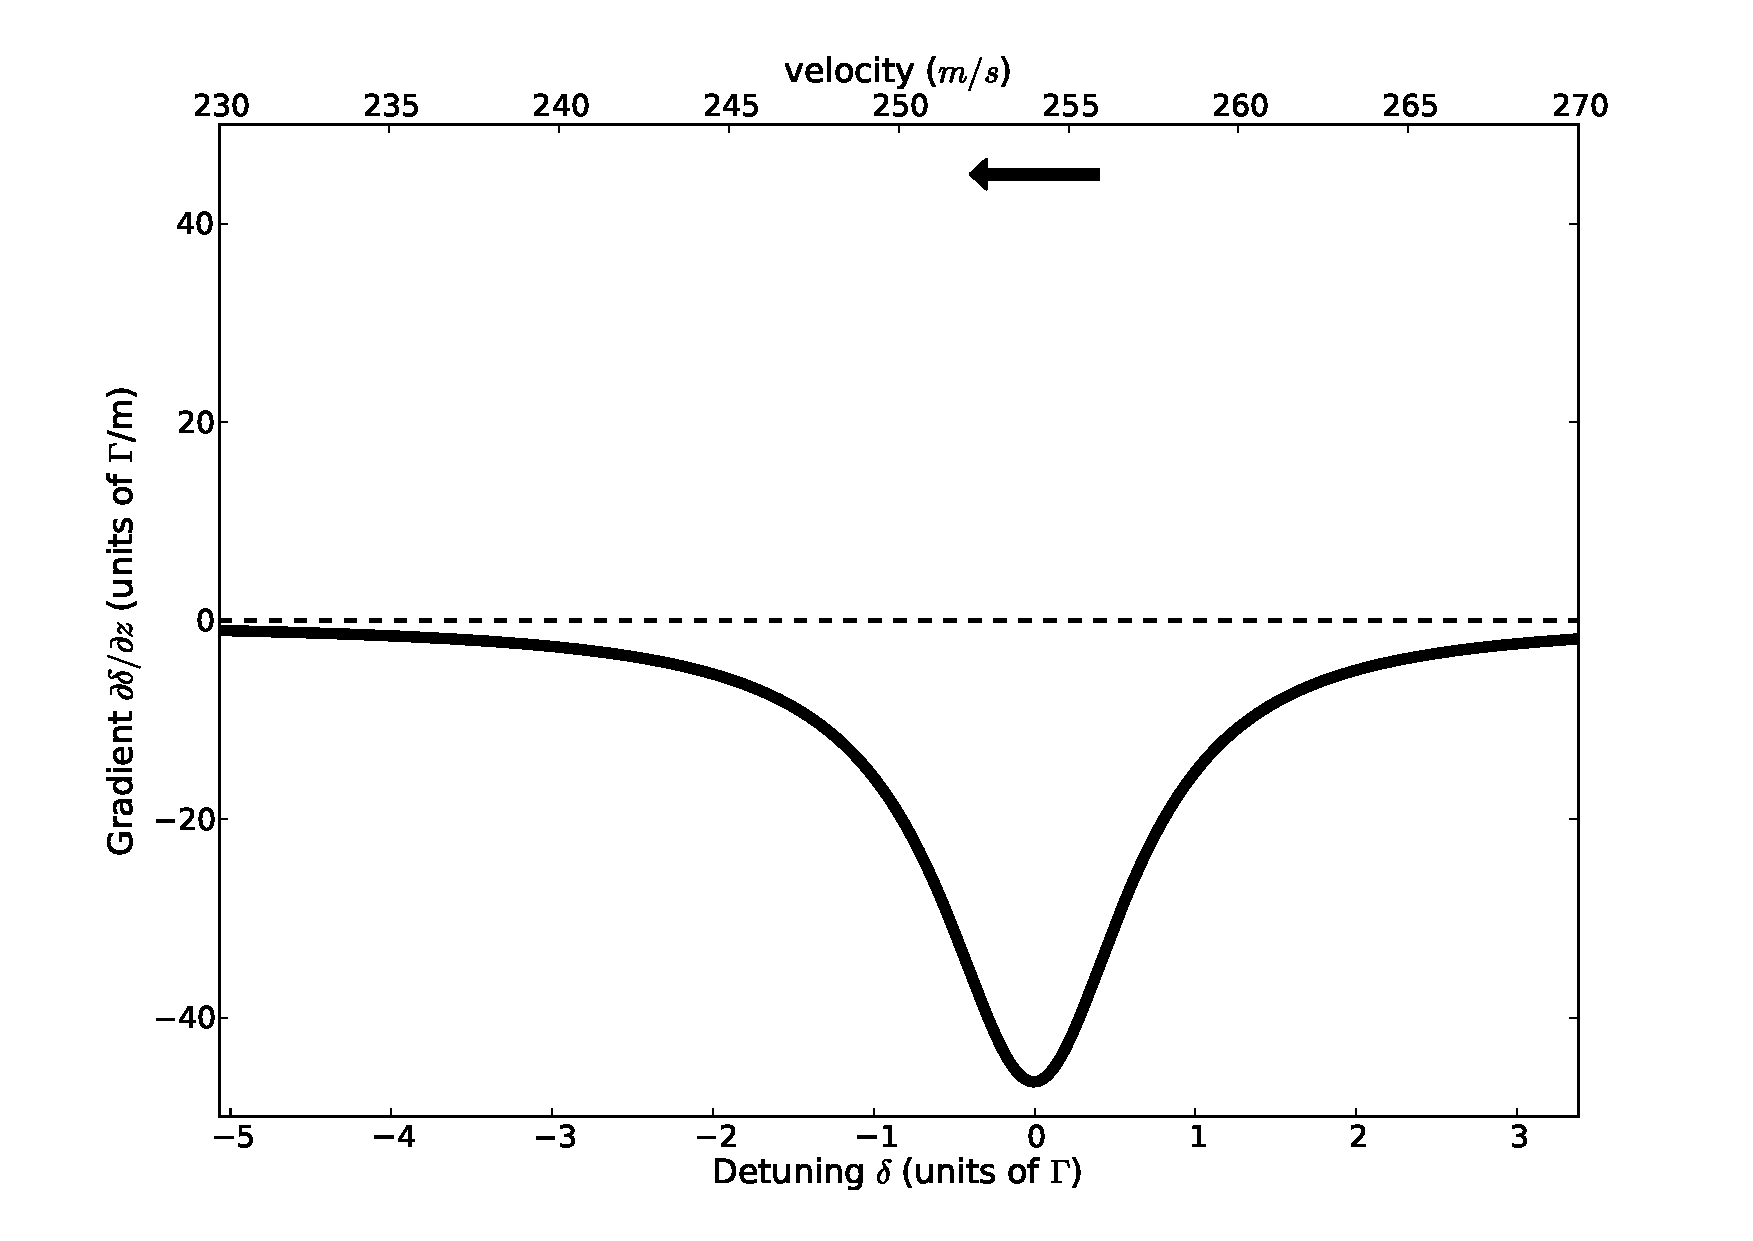
\includegraphics[width=1.0\textwidth]{detu1}
\caption{The spatial gradient of detuning $\delta$ with $\partial B/\partial z=0$ at $z=0$, $v_0 = 254~m/s$, $\eta = 0.5$ and $s = 1$. The arrow means that over the whole whole plotted range, the detuning is decreasing (going red).}
\label{fig:dddz1}
\end{figure}

Figure \ref{fig:dddz2} is a similar plot using the same parameters except for the magnetic field, where $B_{\rm ideal}$ is used as defined in Eq. \ref{eq:bideal}, with its field gradient. Now $\partial \delta / \partial z \geq 0$, meaning the detuning is moving to the blue (because of the change in $B$). There's one special point (for the given parameters) near $\delta = 0$ where $\partial \delta / \partial z = 0$, that is the detuning will be constant. Since $B$ is changing, this implies change in $v$ as well, and given the signs of the changes, implies deceleration.

\begin{figure}[htb]
\centering
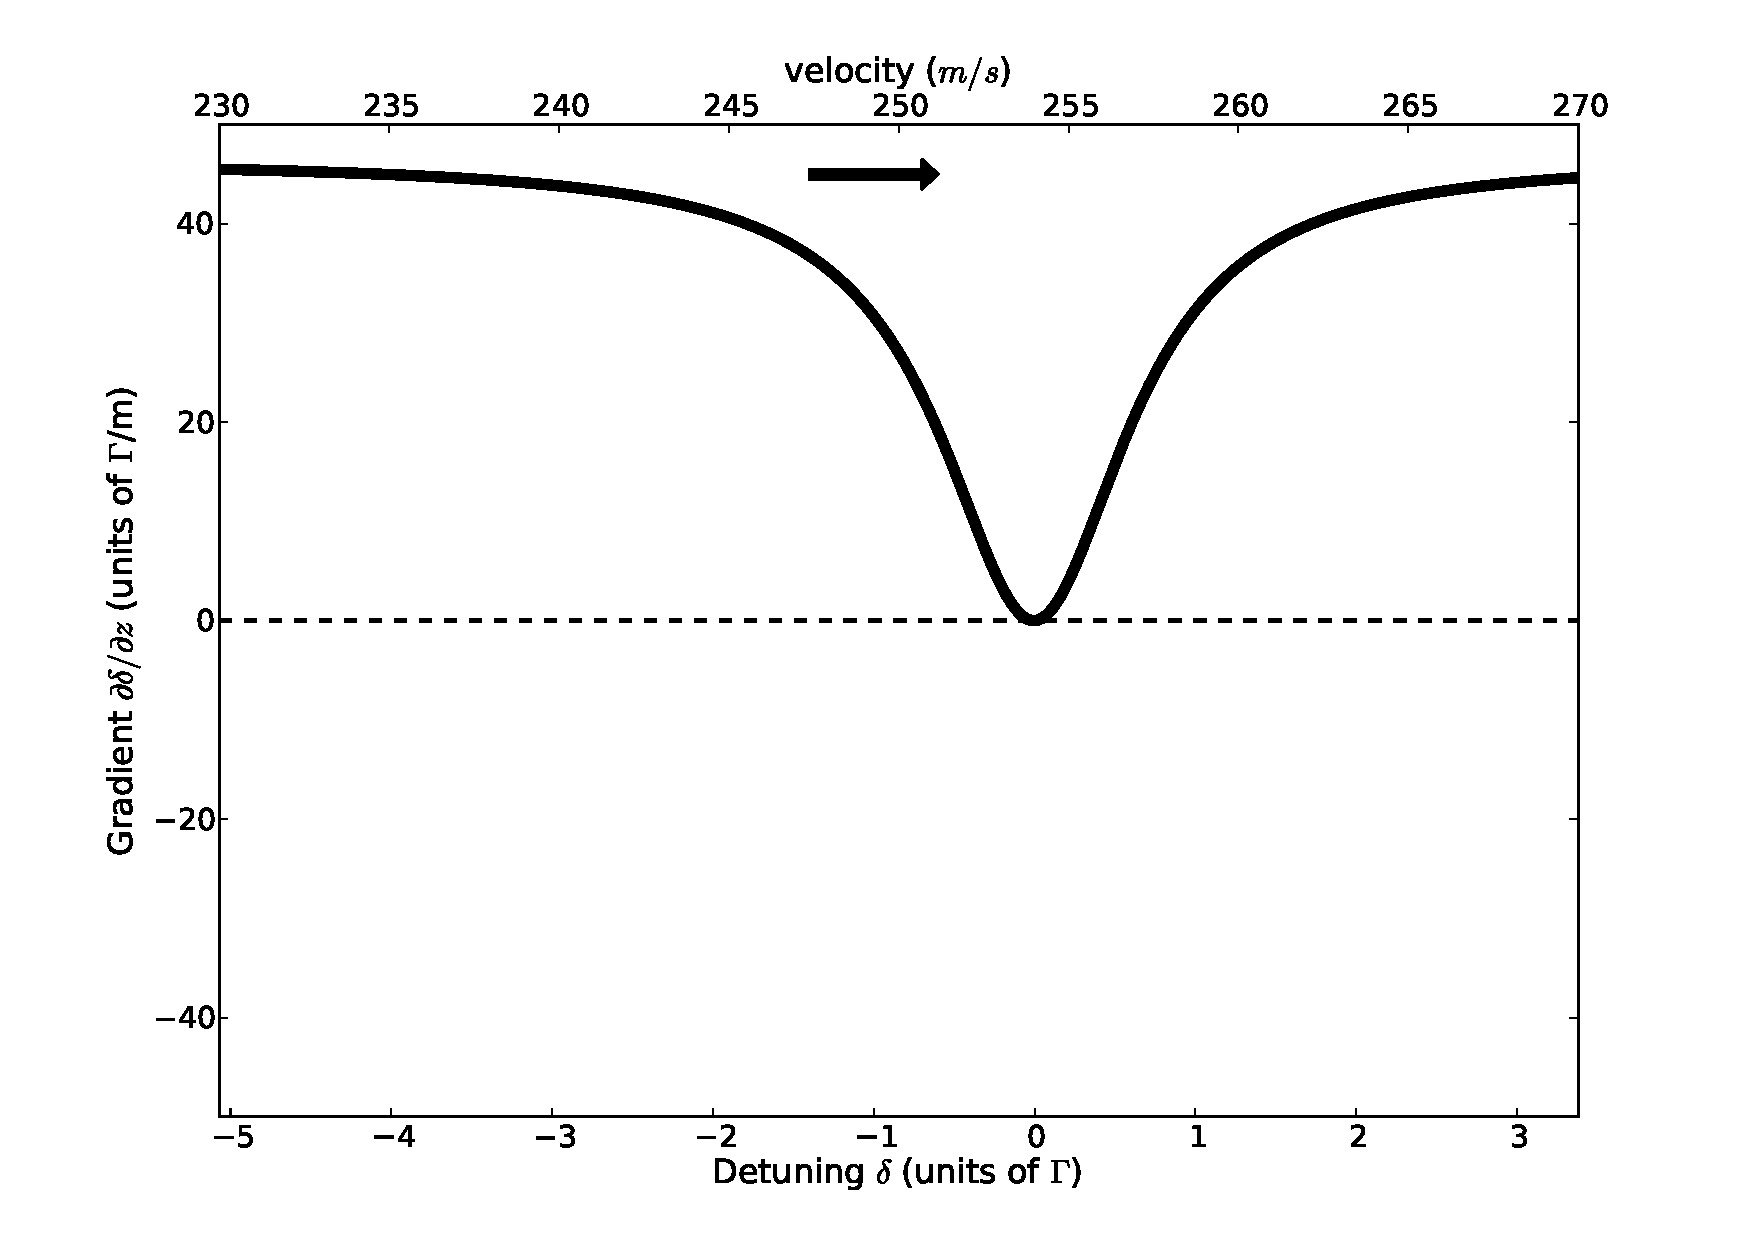
\includegraphics[width=1.0\textwidth]{detu2}
\caption{As Fig. \ref{fig:dddz1} but with $B=B_{\rm ideal}$. The arrow means that over the whole range the detuning is increasing (going blue). Exception is near $\delta = 0$ where there is a fixed point.}
\label{fig:dddz2}
\end{figure}

\begin{figure}[htb]
\centering
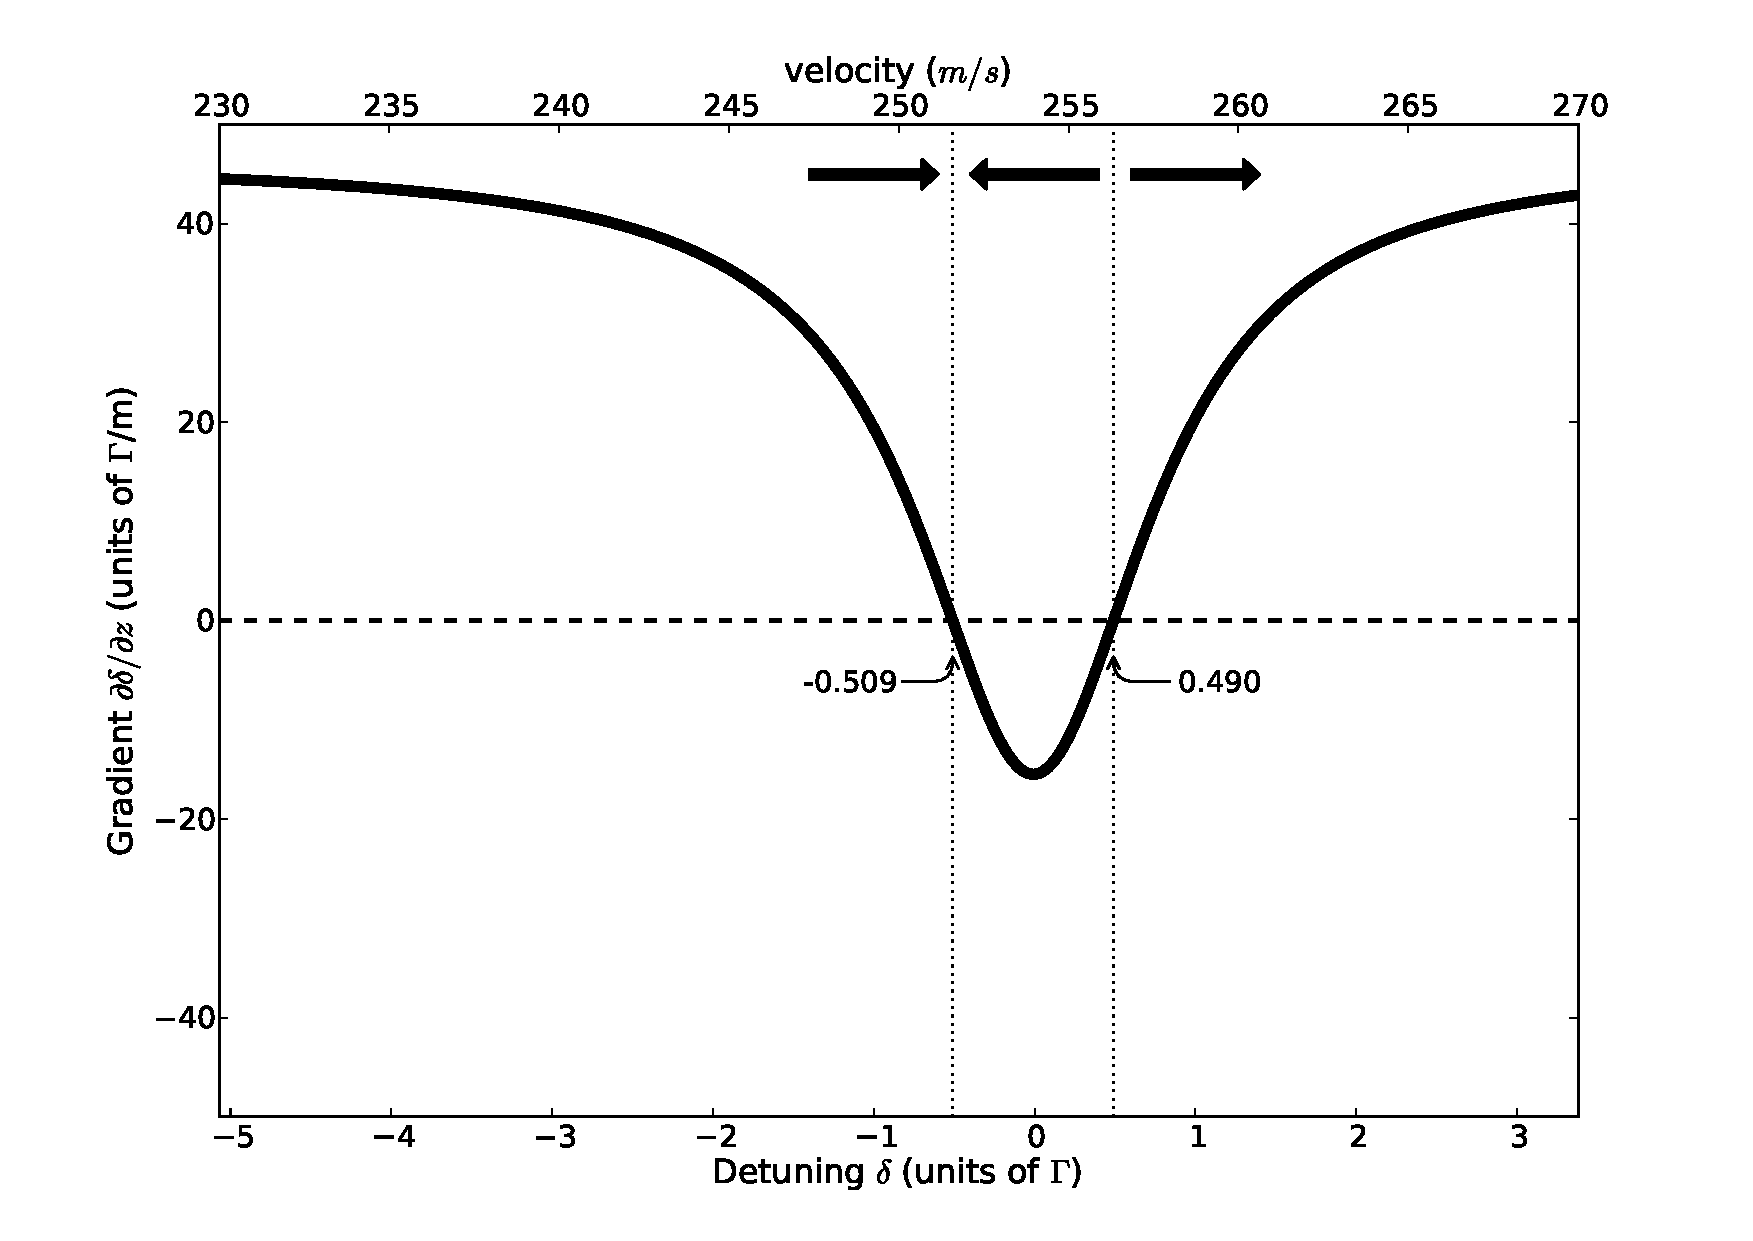
\includegraphics[width=1.0\textwidth]{detu3}
\caption{As Fig. \ref{fig:dddz2} but with $s = 2$, which means higher laser intensity. The line is widened and its height has increased. Now there is a true stable fixed point near $\delta = -0.5 \Gamma$ and an unstable fix point near $\delta = 0.5 \Gamma$. Further increase of laser intensity will push the fixed points away from $\delta = 0$.}
\label{fig:dddz3}
\end{figure}

The zero crossing can be calculated analytically by reorganizing Equation \ref{eq:dddz}. We can make the following substitutions for notational convenience:
\begin{eqnarray}
v &=& \frac{1}{k}\left(\delta - \Delta + \frac{\mu'}{\hbar}B\right) \\
A &=& \frac{\mu'}{\hbar}B \\
X &=& A - \Delta \\
Y &=& 1+s \\
Z &=& \frac{4}{\Gamma^2} \\
W &=& - \frac{\hbar k^3 \Gamma s}{2 m}.
\end{eqnarray}
The detuning $\delta$ can then be expressed as
\begin{equation}
\delta^3 + X \delta^2 + \frac{Y}{z} \delta + \frac{A X Y - W}{A Z}= 0
\end{equation}
which is just a standard cubic equation. The displayed 2 roots (out of the 3) of Figure \ref{fig:dddz3} are calculated with this method.

\section{Construction}

\subsection{Simulation}

Here are the simulation results, and our choice for the used design

\subsection{Assembly}

Here it comes the summary of assembly and the final design parameters



\bibliographystyle{plain}
\bibliography{zeeman}
\end{document}